%\chapter{The Basics of Loading and Manipulating Data}
\chapter{The Invocation and Metamorphosis of Data}

\IMFellEnglish
\lettrine[lines=5, realheight]{K}{NOWLEDGE} is power as they say, but data—data is something else entirely. It is the ghost in the machine, the thing lurking beneath the surface, waiting for you to look too close. Heed this warning: The data frame, and its accursed successor the tibble, are your most loyal servants \ldots{} and your most treacherous foes. Treat them with reverence, for a single misstep may awaken errors best left entombed.

\normalfont

Chapter 1 had stated that \glspl{data frame} are essential for keeping a host of related information stored in a well organized manner that is easy to manipulate. When printed to the console, data frames present information in a familiar spreadsheet-like structure that can be created, subset, and altered in various ways (see section \ref{sec:data_frames} for details). Moreover, in chapter 1, we saw how a data frame can be constructed by manually entering values with R code. And, for all but the smallest of data sets, this method, while simple, is both time-consuming and highly prone to error. A better strategy is to take an existing file of information and import that directly into R as a data frame or, depending on the nature of the data and what needs to be done with it, as a list, matrix, array, or table. Though, a data frame is usually going to be the optimal choice and will be the primary focus of this chapter.

Data can come in all manner of different layouts and file formats and, in this respect, R has the ability to handle pretty much any scenario that might arise. This chapter will be working under the assumption that the kind of data that you need to work with is in a conventional ``spreadsheet-style'' of format. That is to say, like the \R{msleep} data used in Chapter 2, there are sets of rows and columns, with each cell containing just a single value.

\section{Spreadsheet Software}
\label{sec:spreadsheet_soft}

Given the ubiquity of spreadsheet software, it is important to discuss its use and why R offers a preferable alternative for data analysis. Most spreadsheet applications have their own specific file type that is tailored to its unique purpose and platform. For instance, \textit{Microsoft's Excel} spreadsheet application has its own proprietary format called the \texttt{.xlsx} file format. The awful stock spreadsheet application on Macintosh computers, called \textit{Numbers}, uses the \texttt{.NUMBERS} file format. And if you use an open-source spreadsheet software like \textit{Libre Office's Calc} application, you may be familiar with the \texttt{.ods} file format.

As everyone who is reading this doubtlessly appreciates, spreadsheet applications like Microsoft's Excel, Numbers, Libre Office's Calc, etc., do more than just structure your data in a big table.  They allow you to do things like perform calculations, adjust cell colours, add images, insert comments, etc. And all of this is saved, in one form or another, as information inside the specific file associated with that software. These features make applications like Microsoft's Excel, for instance, a great tool for basic tasks like balancing the household budget.  However, for serious data analysis that requires the use of large data sets and complex or heavy calculations, this kind of software is going to be more of a hindrance than a help. Incorporating all those layers of additional functionality is going to boost file sizes, inflate load times, limit the amount of information the spreadsheet can hold, and increase the chance of a glitch occurring. Additionally, and most importantly, both the analyses and the data are all contained within the same file, which makes it very easy to irrevocably damage your original data set, often without even realizing it. The fact is, we should care about analysing our data efficiently and safely, not making it look pretty in what amounts to a fancy table, and this is one of the key benefits of using R.

From the point of view of R, a spreadsheet is just a way of displaying the raw information to be analysed and nothing more. The analysis of that information is what R does. Technically then, we should not be referring to something as a ``spreadsheet file,'' but rather a ``data file.'' The spreadsheet aspect of all of this is more about how the data is structured for our viewing as humans. However, data does not necessarily need to be viewed as a spreadsheet - it can be viewed in all kinds of different ways. It is just that a spreadsheet is usually the most convenient and intuitive way to view it and talk about it.

\section{Using an Ethical File Format}
\label{sec:ethical_file}

As noted above, there are a variety of different spreadsheet file types data could be formatted as (\texttt{.xlsx}, \texttt{.ods}, \texttt{.wks}, etc.). To remain consistent with open-science principles \parencite{UNESCO_open_sci}, best practice dictates that you work with your data in a file format that is both universally recognized across applications and will also stand the test of time in terms of compatibility.  In other words, we want to (ideally) work with a file format that has no immediate risk of becoming obsolete and can be read by multiple computers on multiple platforms without forcing the user to pay for some proprietary application. Along these lines, the most widely used and recognized format is the \texttt{.csv} file format.

\section{The .CSV Format}

``CSV'' stands for ``comma separated values.'' It gets its name from the fact that it is, quite literally, nothing more than a generic text document that uses commas to denote a tabular (spreadsheet) structure in the data.\footnote{``Tabular'' and ``spreadsheet'' mean the same thing here.} This is easiest to see with an example. The GitHub account for this book contains a repository with a file called \R{skull\_cap\_partial\_wide.csv}, located at the following URL:

\begin{center}
\url{https://github.com/statistical-grimoire/thomson-randallmaciver-1905}
\end{center}

\noindent
In the repository, you will see a list of files followed by a README document describing the contents of the repository. Clicking on the file name \R{skull\_cap\_partial\_wide.csv} will open a spreadsheet-style view of that file. This display presents the estimated cranial capacities (in cubic centimetres) for 1,449 ancient Egyptian skulls,\footnote{This is not necessarily a statistic anyone should care about, but Ancient Egypt is really cool and skulls are metal AF. Also, for any Americans reading this, 1 centimetre is equal to 1.181 barleycorns.} and is actually only a subset of a much larger dataset.\footnote{\R{Thomson\_Randall-MacIver\_1905.csv}} These skulls span numerous historical periods, ranging from Egypt's early predynastic era to its Roman occupation.

Upon opening the file on GitHub, the contents appear in a standard tabular format, resembling a typical spreadsheet (see Table \ref{tab:skulls_wide} for an example displaying the first ten rows). With the exception of the columns labelled \R{sex} and \R{predynastic}, each column header corresponds to the starting year of an approximate date range, as reported by the original authors. The prefix \textit{c} denotes \textit{circa} (meaning ``approximately''), followed by a year and the abbreviation \textit{BC} (``Before Christ''), reflecting the historical dating conventions employed by the original authors. A more contemporary and inclusive alternative would be \textit{BCE} (``Before Common Era''). The term \textit{predynastic} refers to periods preceding the earliest recorded Egyptian dynasties, which, at the time of \citeauthor{Thomson1905}'s (\citeyear{Thomson1905}) research, were not yet clearly established or reliably dated.

\vspace{1em}

\begin{table}[!h]
\centering
\resizebox{\textwidth}{!}{
\begin{tabular}{lrrrrrrrrrr}
\toprule
sex & predynastic & c4800BC & c4200BC & c4000BC & c3500BC & c2780BC & c1590BC & c378BC & c331BC & c3700BC\\
\midrule
\cellcolor{gray!10}{Male} & \cellcolor{gray!10}{1370} & \cellcolor{gray!10}{1410} & \cellcolor{gray!10}{1320} & \cellcolor{gray!10}{1445} & \cellcolor{gray!10}{1395} & \cellcolor{gray!10}{1425} & \cellcolor{gray!10}{1440} & \cellcolor{gray!10}{1310} & \cellcolor{gray!10}{1450} & \cellcolor{gray!10}{NA}\\
Male & 1250 & 1445 & 1565 & 1540 & 1420 & 1505 & 1355 & 1395 & 1460 & NA\\
\cellcolor{gray!10}{Male} & \cellcolor{gray!10}{1430} & \cellcolor{gray!10}{1440} & \cellcolor{gray!10}{1600} & \cellcolor{gray!10}{1565} & \cellcolor{gray!10}{1380} & \cellcolor{gray!10}{1360} & \cellcolor{gray!10}{1490} & \cellcolor{gray!10}{1360} & \cellcolor{gray!10}{1360} & \cellcolor{gray!10}{NA}\\
Male & 1350 & 1340 & 1460 & 1710 & 1260 & 1385 & 1425 & 1485 & 1410 & NA\\
\cellcolor{gray!10}{Male} & \cellcolor{gray!10}{1130} & \cellcolor{gray!10}{1460} & \cellcolor{gray!10}{1520} & \cellcolor{gray!10}{1690} & \cellcolor{gray!10}{1285} & \cellcolor{gray!10}{1350} & \cellcolor{gray!10}{1380} & \cellcolor{gray!10}{1365} & \cellcolor{gray!10}{1215} & \cellcolor{gray!10}{NA}\\
\addlinespace
Male & 1670 & 1290 & 1440 & 1775 & 1505 & 1440 & 1490 & 1220 & 1320 & NA\\
\cellcolor{gray!10}{Male} & \cellcolor{gray!10}{1195} & \cellcolor{gray!10}{1290} & \cellcolor{gray!10}{1740} & \cellcolor{gray!10}{1390} & \cellcolor{gray!10}{1230} & \cellcolor{gray!10}{1400} & \cellcolor{gray!10}{1385} & \cellcolor{gray!10}{1195} & \cellcolor{gray!10}{1550} & \cellcolor{gray!10}{NA}\\
Male & 1500 & 1385 & 1410 & 1620 & 1250 & 1255 & 1270 & 1410 & 1320 & NA\\
\cellcolor{gray!10}{Male} & \cellcolor{gray!10}{1325} & \cellcolor{gray!10}{1290} & \cellcolor{gray!10}{1510} & \cellcolor{gray!10}{1500} & \cellcolor{gray!10}{1315} & \cellcolor{gray!10}{1450} & \cellcolor{gray!10}{1585} & \cellcolor{gray!10}{1370} & \cellcolor{gray!10}{1460} & \cellcolor{gray!10}{NA}\\
Male & 1480 & 1565 & 1550 & 1255 & 1360 & 1310 & 1330 & 1365 & 1560 & NA\\
\bottomrule
\end{tabular}}
\caption{First ten rows of \R{skull\_cap\_partial\_wide.csv}, displaying estimated cranial capacity (cm\textsuperscript{3}).}
\label{tab:skulls_wide}
\end{table}





While GitHub nicely formats the file as a spreadsheet for viewing, the actual raw data consists of nothing more than a basic text document that separates individual values with a comma. We can see this more clearly if we click the button on GitHub labelled ``Raw'' which will present the file in its unaltered (i.e., raw) text format. The first 10 rows can be seen below:

\vspace{1em}

\begin{listing}[H]
\begin{raw}
sex,predynastic,c4800BC,c4200BC,c4000BC,c3700BC,c3500BC,c2780BC,c1590BC,c378BC,c331BC
Male,1370,1410,1320,1445,,1395,1425,1440,1310,1450
Male,1250,1445,1565,1540,,1420,1505,1355,1395,1460
Male,1430,1440,1600,1565,,1380,1360,1490,1360,1360
Male,1350,1340,1460,1710,,1260,1385,1425,1485,1410
Male,1130,1460,1520,1690,,1285,1350,1380,1365,1215
Male,1670,1290,1440,1775,,1505,1440,1490,1220,1320
Male,1195,1290,1740,1390,,1230,1400,1385,1195,1550
Male,1500,1385,1410,1620,,1250,1255,1270,1410,1320
Male,1325,1290,1510,1500,,1315,1450,1585,1370,1460
Male,1480,1565,1550,1255,,1360,1310,1330,1365,1560
\end{raw}
\caption*{Example of the \R{skull\_cap\_partial\_wide.csv} data file displayed in its raw text format. Only the first ten rows are shown.}
\end{listing}

Comparing the two versions it can readily be seen how the commas are functioning. They separate individual columns and each new line represents a new row in the spreadsheet. This not only makes it easy to read \texttt{.csv} files within a basic text editor, but create them as well. Just save (or rename) the text document with a \texttt{.csv} file extension (which you may need to configure your computer to display). Alternatively, if you have a good spreadsheet software on your computer, it will have the ability to \textit{``Save As''} a \texttt{.csv} file or \textit{``Export''} to one. For instance, the save menu of Microsoft Excel will present the user with a drop down list of potential file types it can save as and (as of writing this) has four different versions of \texttt{.csv} files (the best option is the one labelled ``UTF-8 Comma delimited''). By contrast the Numbers application on a Mac will not permit a spreadsheet to save as anything other than a \texttt{.NUMBERS} file, but will allow you to export your saved spreadsheet as a \texttt{.csv}. Just select \textit{File $\rightarrow$ Export To $\rightarrow$ CSV.}

\clearpage

\section{Delimiters}

In the case of the \R{skull\_cap\_partial\_wide.csv} file, the comma is functioning as a \gls{delimiter}; which is to say it is a character that defines the limits of (i.e., it ``delimits'') individual values. Commas are not the only characters that can be used to delimit, any character can technically be used. Other common delimiters include semicolons (;) and tab-key spaces. Semicolons are often used when the data is logged with commas representing decimal points instead of periods (e.g., 13.666 = 13,666), which is a frequent practice in many countries. Oddly, when a delimited file uses semicolons, it is still often given a \texttt{.csv} file extension despite it being a completely different character.  In R, to avoid confusion, the convention is to refer to these semicolon delimited files as \R{csv2} files in function names (e.g., \R{read\_csv()} would use a comma to delimit whereas \R{read\_csv2()} would use a semicolon).

Tab spaces (i.e., pressing ``tab'' on your keyboard), are also frequently employed as a delimiter, but these are usually denoted as \texttt{.tsv} files (i.e., tab separated values). In fact, the name for the keyboard key ``tab'' comes from the the verb ``tabulate'' because the key facilitated easier generation of tables when working on a typewriter. Prior to the tab key's development, the space bar had to be repeatedly pressed to advance the typewriter's carriage to align columns appropriately. 

If you were to save the \R{skull\_cap\_partial\_wide.csv} data set as a \texttt{.tsv} file and open it within a generic text editor, you would see something very similar to the following ...

\vspace{1em}

\begin{listing}[H]
\begin{raw}
sex	predynastic	c4800BC	c4200BC	c4000BC	c3700BC	c3500BC	c2780BC
Male	1370	1410	1320	1445	NA	1395	1425	1440	1310	1450
Male	1250	1445	1565	1540	NA	1420	1505	1355	1395	1460
Male	1430	1440	1600	1565	NA	1380	1360	1490	1360	1360
Male	1350	1340	1460	1710	NA	1260	1385	1425	1485	1410
Male	1130	1460	1520	1690	NA	1285	1350	1380	1365	1215
Male	1670	1290	1440	1775	NA	1505	1440	1490	1220	1320
Male	1195	1290	1740	1390	NA	1230	1400	1385	1195	1550
Male	1500	1385	1410	1620	NA	1250	1255	1270	1410	1320
Male	1325	1290	1510	1500	NA	1315	1450	1585	1370	1460
Male	1480	1565	1550	1255	NA	1360	1310	1330	1365	1560
\end{raw}
\caption*{Excerpt of the \R{skull\_cap\_partial\_wide.csv} file displayed in raw text format as if it were a \texttt{.tsv}. Only the first 10 rows are shown; the last three column headers (\texttt{c1590BC}, \texttt{c378BC}, and \texttt{c331BC}) are omitted for space.}
\end{listing}

\noindent Notice that the tabular separation gives the file a much more grid-like aesthetic that is easier to read. Incorporating spaces into the text file can be used to further refine the alignment.

\section{Reading a CSV File into R}

Now that we have a good sense of what a \texttt{.csv} file is, we should discuss how to load it into R as a data frame object so we can conduct our analyses. To begin with, you should download \R{skull\_cap\_partial\_wide.csv} from the aforementioned GitHub repo by simply clicking the ``down arrow'' icon labelled ``\textit{Download raw file.}'' Once downloaded, simply place the file inside your working directory.\footnote{If you are unsure what a ``working directory'' is see section \ref{sec:dir}} Depending on the browser you are using you may have to hunt around for the download option. For instance, if you are using Safari, you may have to select ``more file actions.''

With the file in its appropriate location you can simply run the function \R{read\_csv()} and give it the full name (with extension) of your file as a character string. This will create a data frame object in R. However, \R{read\_csv()} is a function that belongs to the \textit{readr} package which is part of the \textit{tidyverse}, so if you do not have the \textit{tidyverse} loaded, this will not work. In order to easily call our loaded data, we will assign it the name \R{skulls}.

\begin{inR}
library(tidyverse)
skulls <- read_csv("skull_cap_partial_wide.csv")
\end{inR}

\begin{outR}
Rows: 343 Columns: 11                                             
── Column specification ──────────────────────────────────────────
Delimiter: ","
chr  (1): sex
dbl (10): predynastic, c4800BC, c4200BC, c4000BC, c3700BC, c35...

i Use `spec()` to retrieve the full column specification for this data.
i Specify the column types or set `show_col_types = FALSE` to quiet this message.
\end{outR}

Running the above code presents us with some useful information about the data set we have loaded.  We can see that it has 343 rows and 11 columns, uses a \R{,} as a delimiter. One column, \R{sex}, consists of character (\R{chr}) values and the remaining 10 columns consist of \R{dbl} values, which is a shorthand way of referring to \textit{double-precision number}. To simplify a complex story, R has multiple types of \textit{numeric} objects; i.e., it has multiple ways of representing a number. A \textit{double}, as its often referred to, is one such representation. If that is confusing, don't worry, what is important to take away from the output is that \R{dbl} means the column contains numeric values (i.e., we can use them to do mathematics).

\clearpage

Running \R{skulls} will print the data frame to the console.

\begin{inR}
skulls
\end{inR}

\begin{outR}
# A tibble: 343 × 11
   sex   predynastic c4800BC c4200BC c4000BC c3700BC c3500BC c2780BC
   <chr>       <dbl>   <dbl>   <dbl>   <dbl>   <dbl>   <dbl>   <dbl>
 1 Male         1370    1410    1320    1445      NA    1395    1425
 2 Male         1250    1445    1565    1540      NA    1420    1505
 3 Male         1430    1440    1600    1565      NA    1380    1360
 4 Male         1350    1340    1460    1710      NA    1260    1385
 5 Male         1130    1460    1520    1690      NA    1285    1350
 6 Male         1670    1290    1440    1775      NA    1505    1440
 7 Male         1195    1290    1740    1390      NA    1230    1400
 8 Male         1500    1385    1410    1620      NA    1250    1255
 9 Male         1325    1290    1510    1500      NA    1315    1450
10 Male         1480    1565    1550    1255      NA    1360    1310
# i 333 more rows
# i 3 more variables: c1590BC <dbl>, c378BC <dbl>, c331BC <dbl>
# i Use `print(n = ...)` to see more rows
\end{outR}

You can now subset and manipulate the data frame \R{skulls} like was done in Chapter 1 when we first discussing data frames (see section \ref{sec:data_frames}). For instance, if we wanted to look at the mean breadth of skulls from the predynastic period, we could simply run:

\begin{inR}
mean(skulls$predynastic, na.rm = TRUE)
\end{inR}
\begin{outR}
[1] 1320.142
\end{outR}

\noindent
One thing that is not apparent from the ten row output is that \textit{all} of the numeric columns contain some missing, \R{NA}, values—hence the need to specify \R{na.rm = TRUE}.

\subsubsection{\texttt{read.csv()} vs. \texttt{read\_csv()}}

To load the \R{skulls} data frame above, we used the function \R{read\_csv()}, which is part of the \textit{tidyverse}. However, base R has a similar function, \R{read.csv()}, that will do essentially the same thing—it will read a \texttt{.csv} file into R. For most use cases there is little advantage to adopting one function over the other but, if you have the \textit{tidyverse} loaded, you may as well use \R{read\_csv()} because it does have some advantages over its predecessor. First, it offers excellent customization options, which are particularly useful when loading very large datasets or merging multiple datasets. Second, it alerts you to any issues encountered during the loading process. Third, it performs much faster under heavy loads than its base R counterpart, even providing a progress bar when reasonable to do so. Finally, instead of a data frame, it stores the data as a \textit{tibble}, which will be discussed later.

\subsection{Reading Other File Types into R}

If your data is delimited by some character other than a comma (e.g., a semicolon, tab, backslash, etc.), there is a more general function that can be employed called \R{read\_delim()} which allows you to specify any delimiter (i.e., separator) using the argument \R{delim}. For instance, we could have loaded the \R{skulls} data in the following way:

\begin{inR}
skulls <- read_delim("Max_Breadth_TRM_1905.csv", delim = ",")
\end{inR}

\vspace{1em}

\noindent
If your text document was separated by semicolons you would just include \R{delim = ";"}, if it was separated using tabs you would just \R{delim = "\textbackslash t"}, and so on. 

One thing that is worth appreciating about delimited files is that their file extension (e.g., the \texttt{.csv} or \texttt{.tsv} at the end of the file name) is irrelevant to how R reads the file. As has been previously emphasized, \texttt{.csv} files and \texttt{.tsv} files for instance, are just generic text documents, nothing more. This means you may see them with the file extension \texttt{.txt}, but that will not impact how any of the above functions operate.

Now, what would you do if you wanted to load a Microsoft Excel spreadsheet file (i.e., a \texttt{.xlsx} file) into R directly? Well as per the discussion on spreadsheets and ethical file formats (see section \ref{sec:spreadsheet_soft} and \ref{sec:ethical_file}), the best practice is to save it as a \texttt{.csv} using Excel and load that new file directly into R. However, should you wish to eschew this advice, the \textit{tidyverse} does have a package called \textit{readxl} with functions that will allow you to do this. This is not part of the nine core packages, so it will need to be loaded using the \R{library()} function. A word of warning is in order though. As well made as the \textit{readxl} package is, reading \texttt{.xlsx} files directly will, almost certainly, cause more problems than it solves. These files are not intended to be read by anything other than Excel and Microsoft does not want them read by anything other than Excel. Thus, by loading the \texttt{.xlsx} file directly into R, you are (computationally speaking) picking an unnecessary fight with Microsoft. Nine times out of ten, you will win that fight thanks to \textit{readxl}, but you will still probably end up with some nasty bruises and scars.

\clearpage

\section{Tibbles vs. Data Frames}

In the output for \R{skulls} (and the \R{msleep} data from chapter 2) you can see that the output printed to the console specifies that we are looking at something called a \gls{tibble}. The output also helpfully displays the dataset's dimensions and the class of object contained within each column. This is in contrast to the data frame created in chapter 1, which did not do any of that for us. In the \textit{tidyverse's} own words, a tibble is a ...

\begin{displayquote}
\headingfont
%\large
modern reimagining of the data.frame, keeping what time has proven to be effective, and throwing out what is not. Tibbles are data.frames that are lazy and surly: they do less (i.e. they don’t change variable names or types, and don’t do partial matching) and complain more (e.g. when a variable does not exist). This forces you to confront problems earlier, typically leading to cleaner, more expressive code. Tibbles also have an enhanced print( ) method which makes them easier to use with large datasets containing complex objects.

- \textit{\url{https://tibble.tidyverse.org/} (2024/07/28)}

\end{displayquote}

In terms of basic usage, tibbles function almost identically to the classic data frame discussed in chapter 1. For instance, with the \textit{tidyverse} loaded, we can re-create chapter 1's data frame as a tibble using an identical syntax.

\begin{inR}
df <- tibble(
  Subject = 1:10,
  Group = c("Exp", "Cont", "Exp", "Cont", "Exp", "Exp",
            "Cont", "Exp", "Cont", "Cont"),
  Value = c(-0.36,  0.28,  1.54,  0.51, -1.28,  1.15,
            -2.22, -0.51,  NA, -1.04)
)

df
\end{inR}

\begin{outR}
# A tibble: 10 × 3
   Subject Group Value
     <int> <chr> <dbl>
 1       1 Exp   -0.36
 2       2 Cont   0.28
 3       3 Exp    1.54
 4       4 Cont   0.51
 5       5 Exp   -1.28
 6       6 Exp    1.15
 7       7 Cont  -2.22
 8       8 Exp   -0.51
 9       9 Cont  NA   
10      10 Cont  -1.04
\end{outR}

\noindent
There are a number of interesting differences between tibbles and data frames, but nothing that merits any in depth discussion for a beginner with R. For the most part they behave identically. However, there is one difference worth mentioning: for tibbles, indexing a single column by specifying row and column values outputs a tibble. For example, suppose we use our index brackets, \R{[ ]}, to isolate the first 5 rows of column 3 in the \R{skulls} data.

\begin{inR}
skulls[1:5, 3]
\end{inR}

\begin{outR}
# A tibble: 5 × 1
  c4800BC
    <dbl>
1    1410
2    1445
3    1440
4    1340
5    1460
\end{outR}

\noindent This seems sensible enough behaviour, but is in contrast to the traditional behaviour of R's data frame which will output a vector unless more than one column is selected.

\begin{inR}
# Using read.csv to load the data as a data frame
skulls_df <- read.csv("skull_cap_partial_wide.csv")

skulls_df[1:5, 3]
\end{inR}

\begin{outR}
[1] 1410 1445 1440 1340 1460
\end{outR}

This may seem to be a trivial distinction; however, operations such as computing the mean of a column are quite common and often require inserting a numeric vector. Consequently, when the output is a tibble rather than a numeric or logical vector, attempting such operations results in an error.

\begin{inR}
mean(skulls[1:5, 3])
\end{inR}

\begin{outR}
[1] NA
Warning message:
In mean.default(skulls[1:5, 3]) :
  argument is not numeric or logical: returning NA
\end{outR}

\noindent However, you can set the argument \R{drop = TRUE} inside the indexing brackets to coerce the output into a vector.

\begin{inR}
skulls[1:5, 3, drop = TRUE]
mean(skulls[1:5, 3, drop = TRUE])
\end{inR}

\begin{outR}
[1] 1410 1445 1440 1340 1460
[1] 1419
\end{outR}

Should the need arise, switching between tibbles and data frames is a simple matter. For example, to convert our tibble \R{skulls} to a data frame, we can simply use the \R{as.data.frame()} function in R.

\begin{inR}
# tibble to data frame
skulls <- as.data.frame(skulls)
skulls
\end{inR}
\begin{outR}
   sex  predynastic c4800BC c4200BC c4000BC c3700BC c3500BC c2780BC
1  Male        1370    1410    1320    1445      NA    1395    1425
2  Male        1250    1445    1565    1540      NA    1420    1505
3  Male        1430    1440    1600    1565      NA    1380    1360
4  Male        1350    1340    1460    1710      NA    1260    1385
5  Male        1130    1460    1520    1690      NA    1285    1350
6  Male        1670    1290    1440    1775      NA    1505    1440
7  Male        1195    1290    1740    1390      NA    1230    1400
8  Male        1500    1385    1410    1620      NA    1250    1255
9  Male        1325    1290    1510    1500      NA    1315    1450
10 Male        1480    1565    1550    1255      NA    1360    1310
...
\end{outR}

\noindent
To convert it back to a tibble:
\begin{inR}
# data frame to tibble
skulls <- as_tibble(skulls)
skulls
\end{inR}
\begin{outR}
# A tibble: 343 × 11
   sex   predynastic c4800BC c4200BC c4000BC c3700BC c3500BC c2780BC
   <chr>       <dbl>   <dbl>   <dbl>   <dbl>   <dbl>   <dbl>   <dbl>
 1 Male         1370    1410    1320    1445      NA    1395    1425
 2 Male         1250    1445    1565    1540      NA    1420    1505
 3 Male         1430    1440    1600    1565      NA    1380    1360
 4 Male         1350    1340    1460    1710      NA    1260    1385
 5 Male         1130    1460    1520    1690      NA    1285    1350
 6 Male         1670    1290    1440    1775      NA    1505    1440
 7 Male         1195    1290    1740    1390      NA    1230    1400
 8 Male         1500    1385    1410    1620      NA    1250    1255
 9 Male         1325    1290    1510    1500      NA    1315    1450
10 Male         1480    1565    1550    1255      NA    1360    1310
# i 333 more rows
# i 3 more variables: c1590BC <dbl>, c378BC <dbl>, c331BC <dbl>
# i Use `print(n = ...)` to see more rows
\end{outR}

\subsection{Displaying Tibbles in the Console}

\subsubsection{Tibble Dimensions}

Given the limited screen space and the large size of most datasets, tibbles are designed to display only the first 10 rows when printed to the console, making it easier for users to work with their data.

Generally, if you want to view an entire data set, the best practice is not to display it in the console but rather use R's \R{View()} function which opens it in a spreadsheet-style window. That being said, many people will still find the number of rows displayed by a tibble within the console lacking, particularly if you are working on anything other than a small laptop. For this reason, the 10 row limit is a behaviour which can be circumvented in various ways. One simple way is to make use of the \R{print()} function. For instance, if we want to display the first 20 rows we can simply run ...

\begin{inR}
print(skulls, n = 20)
\end{inR}

\vspace{1em}

An alternative method is to change R's default display behaviour by setting the minimum number of rows to output using the \R{options()} function.

\begin{inR}
options(pillar.print_min = 20)
skulls
\end{inR}

\vspace{1em}

\noindent
If that method is your preference, then it is usually advisable to place the \R{options()} code at the top of your R script because it only needs to be run once.\footnote{If you are wondering why we specify \R{pillar...} to set rows, it's because \textit{pillar} is a package in the \textit{tidyverse}.}

What if you wanted to display every single row each time you print a tibble? Well, recall that R represents infinity in the positive direction as (\R{Inf}). We can use that to our advantage here:

\begin{inR}
options(pillar.print_min = Inf)
skulls
\end{inR}

\vspace{1em}

What about columns though? Well, interestingly tibbles will actually conform to the size of your console screen.  So if you can only fit five columns on screen, the tibble will only display those five and notify you of the others not displayed beneath the output. This is done to preserve the ``rectangleness'' of the data so it can be visualized appropriately. This also stands in stark contrast to how base R's data frames behave, which will stack columns on top of each other, seemingly with no consideration of column or row space. Admittedly, its nice to have all that information displayed, but it comes at the cost of being difficult for a human to visually parse. That being said, if you wanted your tibbles to behave like this and always display all columns, you can just add an additional argument, \R{pillar.width = Inf}, to the \R{options()} function:

\begin{inR}
options(
  pillar.print_min = 20,
  pillar.width = Inf
)

skulls
\end{inR}

\vspace{1em}

\noindent
However, if you prefer a more temporary solution, you can just add a \R{width} argument to the \R{print()} function. E.g., 

\begin{inR}
print(skulls, n = 20, width = Inf)
\end{inR}

\vspace{1em}

\subsubsection{The Precision and Display of Decimals in Tibbles}
\label{sec:sig_digs}

To save space and facilitate easier reading, both tibbles and data frames will round values with many decimal values. Though, in the case of tibbles, they do not just simply round to a preset number of digits.  To illustrate what tibbles are doing in this respect, recall that R has a built-in constant for $\pi$.

\begin{inR}
pi
\end{inR}
\begin{outR}
[1] 3.141593
\end{outR}

\noindent
Using that, we will create a simple tibble that repeats $\pi$ four times within a single column.

\begin{inR}
pi_df <- tibble(pie = rep(pi, 4))
pi_df
\end{inR}
\begin{outR}
# A tibble: 10 × 1
     pie
   <dbl>
 1  3.14
 2  3.14
 3  3.14
 4  3.14
\end{outR}

\noindent
One thing that will be noticed is that the tibble is only displaying $\pi$ to two decimal places. However, all of the digits still exist in R's memory and any calculations you do will take those unseen digits into account. For instance, if we isolate the first row's value you can see that all the digits of $\pi$ are displayed.

\begin{inR}
print(pi_df$pie[1], digits = 16)
\end{inR}
\begin{outR}
[1] 3.141592653589793
\end{outR}

\noindent
It is important to understand that tibbles do not limit the actual numeric precision of your data. Rather, they format numbers using \gls{significant figures} (also known as \textit{significant digits}) when printing to the console. This helps maintain the clean, rectangular structure of the tibble output, making columns easier to scan.

The way tibbles work with significant figures is slightly different than you may have learned in primary school math class. Everything in front of the decimal point is always displayed, but each number in front of that decimal point uses up a significant figure (a.k.a. a ``sig fig'' or ``sig dig''). For instance, if you had a number like 666.13.  Displaying that to two sig figs would give you 666. Displayed to three sig figs would again be 666. Displayed to four sig figs would be 666.1. Five sig digs would be 666.13. Six sig figs would be 666.130. Seven would be 666.1300, and so on.\footnote{Note that in conventional mathematics, displaying 666.13 to two sig figs would be 670. The first two significant digits are 6 and 6, but the third digit (6) causes rounding up.}

To increase the number of sig figs shown within a tibble we can simply add another argument to the \R{options()} function:

\begin{inR}
options(pillar.sigfig = 16)
pi_df
\end{inR}
\begin{outR}
# A tibble: 10 × 1
                   pie
                 <dbl>
 1 3.141592653589793e0
 2 3.141592653589793e0
 3 3.141592653589793e0
 4 3.141592653589793e0
\end{outR}

\noindent
Because of limitations of 64-bit computing, a tibble is not going let you exceed 16 sig figs and in certain cases will display results in scientific notation. In this case we see some scientific notation, but it is to the power of 0, so it can be ignored.

\clearpage

\section{Wide Data vs. Tidy Data}

\subsection{Wide Data}
\label{sec:wide_data}

Examining the \R{skull\_cap\_partial\_wide.csv} file loaded at the beginning of this chapter, we see that the data is structured logically. The first column represents the presumed sex (male or female) of the skulls in each row, as recorded by \textcite{Thomson1905}. The remaining columns represent skull measurements from a specific period in Egypt's history. Note that the output below displays only the first 8 of 11 columns, and the number of columns visible in your output may vary depending on your screen size.

\begin{inR}
skulls
\end{inR}

\begin{outR}
# A tibble: 343 × 11
   sex   predynastic c4800BC c4200BC c4000BC c3700BC c3500BC c2780BC
   <chr>       <dbl>   <dbl>   <dbl>   <dbl>   <dbl>   <dbl>   <dbl>
 1 Male         1370    1410    1320    1445      NA    1395    1425
 2 Male         1250    1445    1565    1540      NA    1420    1505
 3 Male         1430    1440    1600    1565      NA    1380    1360
 4 Male         1350    1340    1460    1710      NA    1260    1385
 5 Male         1130    1460    1520    1690      NA    1285    1350
 6 Male         1670    1290    1440    1775      NA    1505    1440
 7 Male         1195    1290    1740    1390      NA    1230    1400
 8 Male         1500    1385    1410    1620      NA    1250    1255
 9 Male         1325    1290    1510    1500      NA    1315    1450
10 Male         1480    1565    1550    1255      NA    1360    1310
# i 333 more rows
# i 3 more variables: c1590BC <dbl>, c378BC <dbl>, c331BC <dbl>
# i Use `print(n = ...)` to see more rows
\end{outR}

This style of layout makes it easy to do certain things with the data. For instance, if we wanted to know the mean breadth of skulls \textit{circa} 4800 BCE, we could just run 

\begin{inR}
mean(skulls$c4800BC, na.rm = TRUE)
\end{inR}

\begin{outR}
[1] 1348.831
\end{outR}

If we wanted to calculate the mean of each column, we can use the \R{apply()} function. This function literally \textit{applies} a function of your choosing to either the columns or rows. For example, we might use \R{apply()} to compute the mean of each column. However, the first column (\R{\$sex}) contains character (\R{chr}) values which we cannot take the mean of. Trying to do so will generate an error, so we need to exclude such columns before performing our calculations. We can use what we learned about indexing in chapter 1 to ignore that first column (see section \ref{sec:df_Index}).

\begin{inR}
apply(skulls[, 2:11], MARGIN = 2, FUN = mean, na.rm = TRUE)
\end{inR}

\begin{outR}
predynastic     c4800BC     c4200BC     c4000BC     c3700BC     c3500BC 
   1320.142    1348.831    1434.375    1494.700    1356.429    1336.663 
   
    c2780BC     c1590BC      c378BC      c331BC 
   1308.454    1347.488    1285.781    1318.642 
\end{outR}

\noindent
The argument \R{FUN} specifies what function is applied. The argument \R{MARGIN} specifies whether that function is applied to the rows (\R{1}) or columns (\R{2}). In this case we are applying it to columns, so we specified \R{MARGIN = 2}. \R{na.rm} is of course an argument belonging to the \R{mean()} function, which we need to specify so R knows how to handle the \R{NA} values in the data.

As another example of \R{apply()}, suppose you wanted to know the maximum value contained in each row, ignoring the first column, you could \textit{apply} the function \R{max()} to the \textit{rows}. Since our data has 343 rows, we will produce a vector of 343 elements, of which only the first 130 are shown below.

\begin{inR}
apply(skulls[, 2:11], MARGIN = 1, FUN = max, na.rm = TRUE)
\end{inR}

\begin{outR}
  [1] 1450 1565 1600 1710 1690 1775 1740 1620 1585 1565 1600 1560 1590
 [14] 1575 1630 1670 1570 1510 1525 1475 1610 1460 1475 1570 1485 1560
 [27] 1570 1570 1510 1540 1495 1520 1640 1600 1515 1590 1450 1740 1515
 [40] 1520 1525 1510 1490 1475 1560 1505 1630 1535 1530 1600 1510 1550
 [53] 1560 1590 1480 1570 1615 1510 1610 1430 1585 1610 1660 1470 1570
 [66] 1665 1440 1520 1560 1460 1485 1385 1530 1485 1470 1510 1430 1420
 [79] 1610 1610 1560 1580 1500 1465 1440 1595 1425 1485 1575 1595 1550
 [92] 1720 1535 1370 1400 1345 1630 1340 1400 1420 1455 1380 1530 1480
[105] 1360 1500 1615 1465 1400 1500 1475 1560 1550 1400 1610 1360 1630
[118] 1760 1325 1400 1510 1640 1635 1620 1435 1305 1490 1545 1465 1540
...
\end{outR}

The structure of this dataset is what is commonly referred to as the \gls{wide format}. At first glance, R makes it fairly easy to work with data in this format. However, we have not attempted anything particularly complex yet and, apart from the first column, all the columns are conveniently numeric. Even though this layout might seem intuitive, it is not ideal for many types of analysis or visualization. In fact, the original dataset\footnote{Full data set: \url{https://github.com/statistical-grimoire/thomson-randallmaciver-1905/blob/main/Thomson_Randall-MacIver_1905.csv}} had to be substantially truncated to fit into a usable wide format for our purposes here.

\clearpage

\subsection{Tidy data}

Despite its shortcomings, use of the \textit{wide format} is fairly common and gets its name from the fact that it spreads variables across multiple columns. In this case, we can treat of the different historical periods of the skulls (predynastic, c4800BC, c4200BC, c4000BC, etc.) as a single variable in its own right. We might call this variable simply ``\textit{period}.'' That is to say, c4800BC represents a \textit{period} in Egypt's history, c4200BC represents a \textit{period} in Egypt's history, c4000BC represents a \textit{period} in Egypt's history, and so on. Adjunct to this is a second variable, which we could refer to as the ``\textit{cranial capacity}'' of the skulls. This variable consists of the literal measurements 1370, 1250, 1430, and so on. And of course ``\textit{sex}'' is a variable in this data as well; however, it is not spread across multiple columns the way \textit{period} and \textit{cranial capacity} are. 

When organizing or arranging data, best practices dictate that you \textbf{restrict a single variable to a single column}. In this case, the variable \textit{period} is being spread across ten columns. And the variable \textit{cranial capacity} is found within each of those ten columns. To fix this, we can use the \textit{tidyverse} function \R{pivot\_longer()}.

\begin{inR}
skulls_tidy <- pivot_longer(skulls,
  cols = predynastic : c331BC,
  names_to = "period",
  values_to = "capacity"
)
skulls_tidy
\end{inR}
\begin{outR}
# A tibble: 3,430 × 3
   sex   period      capacity
   <chr> <chr>          <dbl>
 1 Male  predynastic     1370
 2 Male  c4800BC         1410
 3 Male  c4200BC         1320
 4 Male  c4000BC         1445
 5 Male  c3700BC           NA
 6 Male  c3500BC         1395
 7 Male  c2780BC         1425
 8 Male  c1590BC         1440
 9 Male  c378BC          1310
10 Male  c331BC          1450
# i 3,420 more rows
# i Use `print(n = ...)` to see more rows
\end{outR}

Notice a few differences with this pivoted data. There are now considerably more rows in the data, 3,430 vs. 343, and there are two new columns, \R{\$period} and \R{\$capacity} which have replaced the ten different time period columns. In terms of the \R{pivot\_longer()} function we used, the most important argument we specified is \R{cols}, as this defines which columns are going to be collapsed into a single column. The arguments \R{names\_to} and \R{values\_to} just specify the name of the new columns and are not strictly required, but are good practice to include.

In the above code, we used \R{:} to specify a range of columns (from predynastic to c331BC), but we could have instead provided a vector of column names, as shown below:

\begin{inR}
cols <- c(
  predynastic, c4800BC, c4200BC, c4000BC, c3700BC,
  c3500BC, c2780BC, c1590BC, c378BC, c331BC
)
\end{inR}
\vspace{1em}

\noindent It is worth noting that the \textit{tidyverse} has numerous methods for selecting multiple columns simultaneously that do not exist as part of base R. For a rundown of each see the R documentation: \R{?tidyr\_tidy\_select}. Additionally, if you are operating outside of the \textit{tidyverse}, analogous base R functions will usually require column names to be entered as character strings; though, \textit{tidyverse} functions are typically indifferent to this practice. E.g.,

\begin{inR}
cols <- c(
  "predynastic", "c4800BC", "c4200BC", "c4000BC", "c3700BC",
  "c3500BC", "c2780BC", "c1590BC", "c378BC", "c331BC"
)
\end{inR}
\vspace{1em}

By collapsing the 10 period columns into one, the data has now ascended into a sacred arrangement known as \gls{tidy data} (or, as some heretics call it, ``the long format'').  Tidy data is a cornerstone of the \textit{tidyverse's} thaumaturgy and all tidy data adheres to three basic precepts:

\begin{minipage}{\textwidth}

\begin{enumerate}[label=\Roman*.]
\IMFellEnglish
    %\setlength\itemsep{-1em}
    %\large
    \item Each variable is a column; each column is a variable.
    \item Each observation is a row; each row is an observation.
    \item Each value is a cell; each cell is a single value.
\end{enumerate}
\end{minipage}

\noindent
It can be seen that the skull data now satisfies these three standards, as did the \R{msleep} data used in chapter 2. As we progress through the remainder of this chapter, it will become apparent that having your data in this tidy form will greatly facilitate both plotting and analysis. 

Interestingly, because of the restriction that data frames and tibbles have whereby each column needs to contain the same amount of elements, the wide data necessarily had to make use of \R{NA} values. The pivoting that was done to transform the data from wide to tidy preserved those \R{NA} values, but now there is no need for them to keep them in the data (because they just represent a non-existent value). As an example, consider row five:

\clearpage

\begin{inR}
skulls_tidy[5, ]
\end{inR}
\begin{outR}
# A tibble: 1 × 3
  sex   period  capacity
  <chr> <chr>      <dbl>
1 Male  c3700BC       NA
\end{outR}

\noindent
Without a value for \R{\$capacity}, this row conveys no meaningful information. As such, it—and any rows like it—can be safely removed from the dataset.

\begin{inR}
skulls_tidy <- drop_na(skulls_tidy, capacity)
skulls_tidy
\end{inR}
\begin{outR}
# A tibble: 1,449 × 3
   sex   period      capacity
   <chr> <chr>          <dbl>
 1 Male  predynastic     1370
 2 Male  c4800BC         1410
 3 Male  c4200BC         1320
 4 Male  c4000BC         1445
 5 Male  c3500BC         1395
 6 Male  c2780BC         1425
 7 Male  c1590BC         1440
 8 Male  c378BC          1310
 9 Male  c331BC          1450
10 Male  predynastic     1250
# i 1,439 more rows
# i Use `print(n = ...)` to see more rows
\end{outR}

\noindent
The function \R{drop\_na()} simply removes (i.e., ``drops'') any rows that have a \R{NA} value in the columns you specify. Numerous methods exist for removing \R{NA} values, this is merely one means by which to do that that remains true to the \textit{tidyverse's} cannon of spell casting.

\section{Laying Pipe (The \texttt{|>} and \texttt{\%>\%} Operators)}

One of the most significant contributions of the \textit{tidyverse} to R has been its seamless implementation of what is known as `piping' syntax, which allows for an almost otherworldly level of efficiency. However, this is not to say that piping was a concept invented entirely by the \textit{tidyverse}. Rather, the \textit{tidyverse}'s consistent and innovative use of it brought its potential to light, leading to widespread adoption within the R community. The best evidence of this influence is the integration of piping into base R as of \href{https://stat.ethz.ch/pipermail/r-announce/2021/000670.html}{version 4.1.0}, released in 2021.\footnote{Although I have no direct evidence that the \textit{tidyverse} directly motivated the addition of the pipe operator to base R, it seems unlikely to be a coincidence given the ubiquity of \R{\%>\%} and the popularity of the \textit{dplyr} package.} But, for the uninitiated, what exactly is `piping'?

The essence of piping is that you are transferring the output of one thing to another. For instance, suppose we wanted to know the mean cranial capacity across all periods of skulls. We could of course insert the \R{\$capacity} column into the mean function like so ...

\begin{inR}
mean(skulls_tidy$capacity)
\end{inR}
\begin{outR}
[1] 1335.255
\end{outR}

Alternatively, we could ``pipe'' (i.e., transfer) the \R{\$capacity} column in our tidy data to the \R{mean()} function using R's pipe operator \R{|>}

\begin{inR}
skulls_tidy$capacity |> mean()
\end{inR}
\begin{outR}
[1] 1335.255
\end{outR}

\noindent We could then send that output to something like the \R{round()} function.

\begin{inR}
skulls_tidy$capacity |>
  mean() |>
  round(1)
\end{inR}
\begin{outR}
[1] 1335.3
\end{outR}

As another example, suppose we wanted a tidy data frame that only contained skulls from the predynastic period. The standard methodology would be to specify the data frame within the \R{filter()} function, like so ...

\begin{inR}
filter(skulls_tidy, period == "predynastic")
\end{inR}
\begin{outR}
# A tibble: 318 × 3
   sex   period      capacity
   <chr> <chr>          <dbl>
 1 Male  predynastic     1370
 2 Male  predynastic     1250
 3 Male  predynastic     1430
 4 Male  predynastic     1350
 5 Male  predynastic     1130
 6 Male  predynastic     1670
 7 Male  predynastic     1195
 8 Male  predynastic     1500
 9 Male  predynastic     1325
10 Male  predynastic     1480
# i 308 more rows
# i Use `print(n = ...)` to see more rows
\end{outR}

\noindent
Alternatively, we could pipe the data into the \R{filter()} function to achieve the exact same result.

\begin{inR}
skulls_tidy |> filter(period == "predynastic")
\end{inR}

\vspace{1em}

In addition to this, suppose you did not want the \R{\$sex} column inside the output. To achieve this, this output could be further piped into the \textit{tidyverse's} \R{select()} function which allows you to grab specific columns.\footnote{Note that we could obtain the same result by excluding the sex column in the function. i.e., \R{select(-c(sex))}}

\begin{inR}
skulls_tidy |> 
  filter(period == "predynastic") |> 
  select(period, capacity)
\end{inR}
\begin{outR}
# A tibble: 318 × 2
   period      capacity
   <chr>          <dbl>
 1 predynastic     1370
 2 predynastic     1250
 3 predynastic     1430
 4 predynastic     1350
 5 predynastic     1130
 6 predynastic     1670
 7 predynastic     1195
 8 predynastic     1500
 9 predynastic     1325
10 predynastic     1480
# i 308 more rows
# i Use `print(n = ...)` to see more rows
\end{outR}

Now that the logic of piping is clear, it is worth reiterating that the \R{|>} operator is a relatively new arrival in base R. Prior to its introduction in R \href{https://stat.ethz.ch/pipermail/r-announce/2021/000670.html}{version 4.1.0}, the convention would be to use the \textit{tidyverse's} pipe operator \R{\%>\%} instead. This comes from a package called \textit{magrittr} which contains a variety of pipes for different purposes, but the most significant of these is \R{\%>\%}. This was, and to a certain extent still is, the de facto pipe used by the R community at large. However, the recommended wisdom now (by the keepers of the \textit{tidyverse}) is to use base R's pipe and not \textit{magrittr's}. That being said, many are unaware of this update to base R and much of the help documentation on websites like \href{https://stackoverflow.com/}{stack overflow} still use \textit{magrittr's} \R{\%>\%}. In terms of functionality, there is little meaningful difference between \R{|>} and \R{\%>\%} and all of the above code could have been written using \R{\%>\%}.

The above examples nicely show how the pipe operator works, but we should consider a more realistic use case to illustrate its versatility. 

\subsection{Data Manipulation Example}

\subsubsection{Summarising the Data}

The \R{skull\_cap\_partial\_wide.csv} data we loaded earlier was of course in the wide format originally, which is rarely needed. So what we could have done instead is loaded that data in to R using \R{read\_csv}, pipe it to the \R{pivot\_longer()} function, and then pipe that into the \R{drop\_na()} function.

\begin{inR}
skulls <- read_csv("skull_cap_partial_wide.csv") |>
  pivot_longer(
    cols = predynastic:c331BC,
    names_to = "period",
    values_to = "capacity"
  ) |>
  drop_na(capacity)

skulls
\end{inR}
\begin{outR}
# A tibble: 1,449 × 3
   sex   period      capacity
   <chr> <chr>          <dbl>
 1 Male  predynastic     1370
 2 Male  c4800BC         1410
 3 Male  c4200BC         1320
 4 Male  c4000BC         1445
 5 Male  c3500BC         1395
 6 Male  c2780BC         1425
 7 Male  c1590BC         1440
 8 Male  c378BC          1310
 9 Male  c331BC          1450
10 Male  predynastic     1250
# i 1,439 more rows
# i Use `print(n = ...)` to see more rows
\end{outR}

It is worth emphasizing the utility of the pipe operator here: It allowed us to get our data into the form we wanted without creating and calling multiple different objects in memory. Only one object was created, \R{skulls}. Moreover, the ``arrow-like'' notation of the pipe \R{|>} nicely shows the workflow, i.e., logic, of our code.

Now suppose we wanted to compute some summary statistics for this data set.  For instance, maybe we want to know the mean cranial capacity of each period. This is where the \textit{tidyverse's} functions \R{group\_by()} and \R{summarise()} become extremely useful. Both of these functions, as well as the \R{filter()} and \R{select()} functions we have been using, come from a very influential \textit{tidyverse} package called \textit{dplyr}. 

\begin{mdframed}[nobreak = true, style = miscFrame, frametitle = \Large\IMFellEnglish Box 3.1: Why is it called \textit{dplyr}?]
\color{darkgray}
\IMFellEnglish

Generally, the names of R packages are relatively intuitive or are based on an initialism of some kind. The \textit{dplyr} package is an exception to that. The package's strange name is a reference to both pliers (the tool) and a family of functions based around the \R{apply()} function that we briefly used in section \ref{sec:wide_data}. The \enquote{d} refers to data frames. i.e., it is as if you are taking a pair of pliers to data frames.

A common go-to strategy of programmers generally is to use for-loops to do much of the computational grunt work. For-loops just repeatedly execute a set of code until some condition has been satisfied. While for-loops can be used in R, its users often prefer to take a different, more efficient, \enquote{vectorized} approach. The goal is to use what are called \glspl{functional}. These are functions that accept another function as an input and produce a vector as output. That is precisely what the \R{apply()} function and its relatives like \R{lapply}, \R{sapply}, \R{vapply} do. R is incredibly adept at working with vectors, matrices, and arrays, and \textit{dplyr's} functions are all based around a strategy of using functionals for data manipulation.
\end{mdframed}

We will begin with the \R{summarise()} function which is used to create a data frame of summarised information based on columns/variables in your data.

\begin{inR}
skulls |> 
  summarise(m = mean(capacity))
\end{inR}

\begin{outR}
# A tibble: 1 × 1
      m
  <dbl>
1 1335.
\end{outR}

The code we have written is telling the \R{summarise()} function to apply the \R{mean()} function to the \R{\$capacity} column. When it did this, it also created a new data frame\footnote{Yes, yes—I know, \textit{technically} what we created was a \textit{tibble}. But that’s only because \R{skulls} was already a tibble to begin with. For the sake of sanity (mine and yours), I’ll be treating tibbles and data frames as interchangeable for the rest of this book. Purists, feel free to clutch your pearls.} and stored that calculation as a column called \R{\$m} (though, we could have named the column whatever we wanted).

At present, none of this may seem terribly useful; however, we can make it more useful by including the \R{group\_by()} function which will tell R to literally ``group by'' categories found in a different column or set of columns. Specifically, we can tell it to group by \R{\$period} and then summarise the data.

\begin{inR}
skulls |> 
  group_by(period) |> 
  summarise(m = mean(capacity))
\end{inR}
\begin{outR}
# A tibble: 10 × 2
   period          m
   <chr>       <dbl>
 1 c1590BC     1347.
 2 c2780BC     1308.
 3 c331BC      1319.
 4 c3500BC     1337.
 5 c3700BC     1356.
 6 c378BC      1286.
 7 c4000BC     1495.
 8 c4200BC     1434.
 9 c4800BC     1349.
10 predynastic 1320.
\end{outR}

We can now see the mean of each period in the data set and if we wanted, we could create another column, \R{\$n}, showing how many skulls there are in each period total by using the \R{length()} function to count the skulls.

\begin{inR}
skulls |>
  group_by(period) |>
  summarise(
    m = mean(capacity),
    n = length(capacity)
  )
\end{inR}
\begin{outR}
# A tibble: 10 × 3
   period          m     n
   <chr>       <dbl> <int>
 1 c1590BC     1347.   203
 2 c2780BC     1308.   152
 3 c331BC      1319.   232
 4 c3500BC     1337.   315
 5 c3700BC     1356.     7
 6 c378BC      1286.    32
 7 c4000BC     1495.    50
 8 c4200BC     1434.    16
 9 c4800BC     1349.   124
10 predynastic 1320.   318
\end{outR}

If we wanted to add in a column, \R{\$N}, that represented the total amount of skulls across all the periods we could count the number of rows in \R{\$skulls}...

\begin{inR}
nrow(skulls)
\end{inR}
\begin{outR}
[1] 1449
\end{outR}

\noindent
... and include that in the \R{summarise()} function.

\begin{inR}
skulls |>
  group_by(period) |>
  summarise(
    m = mean(capacity),
    n = length(capacity),
    N = nrow(skulls)
  )
\end{inR}

\begin{outR}
# A tibble: 10 × 4
   period          m     n     N
   <chr>       <dbl> <int> <int>
 1 c1590BC     1347.   203  1449
 2 c2780BC     1308.   152  1449
 3 c331BC      1319.   232  1449
 4 c3500BC     1337.   315  1449
 5 c3700BC     1356.     7  1449
 6 c378BC      1286.    32  1449
 7 c4000BC     1495.    50  1449
 8 c4200BC     1434.    16  1449
 9 c4800BC     1349.   124  1449
10 predynastic 1320.   318  1449
\end{outR}

Mathematical operations can also be applied to columns created within the \R{summarise()} function. For instance, historical sources suggest that the ancient Egyptians used a volumetric unit known as the ``heqat,'' primarily for measuring grain, with an estimated value of approximately 4.8 litres \parencite{Clagett1989}. This allows us to convert skull capacities from cubic centimetres to heqats through a simple division. Since 1 litre = 1,000 cm\textsuperscript{3}, it follows that 1 heqat $\approx$ 4,800 cm\textsuperscript{3}. Thus if we wanted the mean and median cranial capacity in heqats we simply run ...

\begin{inR}
skulls |>
  group_by(period) |>
  summarise(
    m = mean(capacity),
    n = length(capacity),
    N = nrow(skulls),
    m_heq = m / 4800,
    med_heq = median(capacity) / 4800
  )
\end{inR}

\clearpage

\begin{outR}
# A tibble: 10 × 6
   period          m     n     N m_heq med_heq
   <chr>       <dbl> <int> <int> <dbl>   <dbl>
 1 c1590BC     1347.   203  1449 0.281   0.280
 2 c2780BC     1308.   152  1449 0.273   0.270
 3 c331BC      1319.   232  1449 0.275   0.275
 4 c3500BC     1337.   315  1449 0.278   0.277
 5 c3700BC     1356.     7  1449 0.283   0.284
 6 c378BC      1286.    32  1449 0.268   0.266
 7 c4000BC     1495.    50  1449 0.311   0.311
 8 c4200BC     1434.    16  1449 0.299   0.306
 9 c4800BC     1349.   124  1449 0.281   0.283
10 predynastic 1320.   318  1449 0.275   0.273
\end{outR}

\noindent
Notice that in the expression \R{m\_heq = m / 4800}, we were able to reuse the previously defined variable \R{m} within the same \R{summarise()} function. This is one of the more especially convenient aspects of this piping approach.

To finish up, lets include the maximum and minimum capacities found in each period. We will also store this as an tibble called \R{skull\_summary}.

\begin{inR}
skull_summary <- skulls |>
  group_by(period) |>
  summarise(
    m = mean(capacity),
    n = length(capacity),
    N = nrow(skulls),
    m_heq = m / 4800,
    med_heq = median(capacity) / 4800,
    min = min(capacity),
    max = max(capacity)
  )
skull_summary
\end{inR}

\clearpage

\begin{outR}
# A tibble: 10 × 8
   period          m     n     N m_heq med_heq   min   max
   <chr>       <dbl> <int> <int> <dbl>   <dbl> <dbl> <dbl>
 1 c1590BC     1347.   203  1449 0.281   0.280  1080  1665
 2 c2780BC     1308.   152  1449 0.273   0.270  1030  1660
 3 c331BC      1319.   232  1449 0.275   0.275  1000  1570
 4 c3500BC     1337.   315  1449 0.278   0.277   965  1760
 5 c3700BC     1356.     7  1449 0.283   0.284  1245  1450
 6 c378BC      1286.    32  1449 0.268   0.266  1095  1550
 7 c4000BC     1495.    50  1449 0.311   0.311  1235  1775
 8 c4200BC     1434.    16  1449 0.299   0.306  1110  1740
 9 c4800BC     1349.   124  1449 0.281   0.283  1110  1640
10 predynastic 1320.   318  1449 0.275   0.273  1050  1710
\end{outR}

\subsubsection{Plotting the Summarised Data}

Now that we have neatly organized these summary statistics inside a tibble, we can visualize them. Since the \R{\$period} column contains ten discrete categories, a bar plot is a basic natural choice for representing these data, so that is what we will create.

The basic logic of plotting has been discussed at length in chapter 2, and this discussion will follow from that.\footnote{In other words, if you haven't read chapter 2, go back and do that.} The first step will be to give \textit{ggplot2} the data and tell it which columns to map to the $x$ and $y$ axis respectively. Then we will add the \R{geom\_bar()} function to this. In this case, we are going to display the mean (i.e., column \R{\$m}) on the y-axis because that is a fairly standard practice many people will be familiar with. Though, it is worth remembering that any of the other numeric (\R{<dbl>}) columns could be used as well.

\begin{inR}
ggplot(skull_summary, aes(x = period, y = m)) +
  geom_bar(stat = "identity") +
  labs(x = "Period", y = "Cranial Capacity (cm³)")
\end{inR}

\vspace{2em}

\begin{figure}[H]
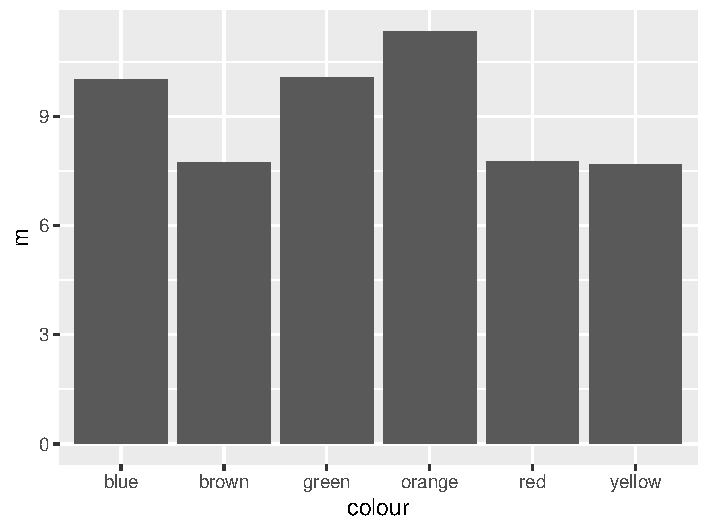
\includegraphics[scale = .75]{graphics/ch3Figs/bar_1.pdf}
\end{figure}

The argument \R{stat = "identity"} is simply telling \textit{ggplot2} to use the values within the \R{skull\_summary} tibble to create the bars.  We needed to specify this because \textit{ggplot2} has the ability to take the raw data directly (e.g., \R{skulls}) and perform its own summary calculations. However, we do not need it to do that in this particular case, hence why we included this argument.

At the moment, going from left to right, the time periods confusingly appear in a non-chronological order. So how do we fix that? This is where the concept of \textit{factors} becomes essential.

\section{Factors}

In statistics, we often refer to a categorical variable as a \gls{factor}. Factors consist of different \glspl{level}, which correspond to the unique categories that variable can take.

For example, in our tidy data, the variable \R{\$period} can be considered a factor. Each distinct time period in that column—such as \R{predynastic}, \R{c4800BC}, \R{c4200BC}, \R{c4000BC}, and so on—represents a different level of the factor. That is, the factor named \R{\$period} has multiple levels, one for each unique period label.

To summarize: in tidy data, you can think of a ``factor'' as essentially a categorical variable (or column), and a ``level'' as one of its possible categories. Just beware that this terminology is specific to tidy data layouts.\footnote{While ``factors'' have a more technical definition in statistics—particularly in the context of experimental design and modelling—this simplified description is sufficient for our current purposes.}

\clearpage

{
\begin{itemize}
  \setlength\itemsep{-1em}
    \item Factor = column
    \item Level = category within a column
\end{itemize}
}

\noindent
If we examine \R{skulls}:

\begin{inR}
skulls
\end{inR}
\begin{outR}
# A tibble: 1,449 × 3
   sex   period      capacity
   <chr> <chr>          <dbl>
 1 Male  predynastic     1370
 2 Male  c4800BC         1410
 3 Male  c4200BC         1320
 4 Male  c4000BC         1445
 5 Male  c3500BC         1395
 6 Male  c2780BC         1425
 7 Male  c1590BC         1440
 8 Male  c378BC          1310
 9 Male  c331BC          1450
10 Male  predynastic     1250
# i 1,439 more rows
# i Use `print(n = ...)` to see more rows
\end{outR}

\noindent
You can see that the output is telling us that the \R{\$period} column is a character vector (notice the \R{<chr>}). In other words, R does not know that \R{predynastic}, \R{c4800BC}, \R{c4200BC}, etc. are categories. It just sees 1,449 individual character values in that particular column. For the purpose of plotting and analyses, it is important that R understands that these are levels of a factor (i.e., it is important that it treats these as categories). We can easily tell R that a particular column is a factor using the function \R{factor()}.\footnote{Technically, when we use this function we are replacing an existing column with a new column that happens to be a class of object called a factor. We are not really ``telling'' R it is a factor, we are ``creating'' a factor - but that's just a nitpicky semantic issue.}

\begin{inR}
skulls$period <- factor(skulls$period)
skulls
\end{inR}
\begin{outR}
# A tibble: 1,449 × 3
   sex   period      capacity
   <chr> <fct>          <dbl>
 1 Male  predynastic     1370
 2 Male  c4800BC         1410
 3 Male  c4200BC         1320
 4 Male  c4000BC         1445
 5 Male  c3500BC         1395
 6 Male  c2780BC         1425
 7 Male  c1590BC         1440
 8 Male  c378BC          1310
 9 Male  c331BC          1450
10 Male  predynastic     1250
# i 1,439 more rows
# i Use `print(n = ...)` to see more rows
\end{outR}

\noindent
Notice that the \R{\$period} column is now labelled as \R{<fct>}, which stands for ``factor.'' Additionally, if we isolate this column, the ten levels of the factor are displayed at the bottom of the output.

\begin{inR}
skulls$period
\end{inR}
\begin{outR}
...
10 Levels: c1590BC c2780BC c331BC c3500BC c3700BC ... predynastic
\end{outR}

\noindent
While this implicit listing is convenient, a better and more deliberate way to view the levels of a factor is to use the \R{levels()} function.

\begin{inR}
levels(skulls$period)
\end{inR}
\begin{outR}
 [1] "c1590BC"     "c2780BC"     "c331BC"      "c3500BC"     "c3700BC"    
 [6] "c378BC"      "c4000BC"     "c4200BC"     "c4800BC"     "predynastic"
\end{outR}

\subsection{Ordering Levels}

Discerning readers may have noticed that the order of the levels shown match the order of the bars in the graph we created. This is not a coincidence. Whenever you use \textit{ggplot2} to plot or \textit{dplyr} to summarize categorical data, these packages quietly convert the relevant columns into factors behind the scenes when necessary. By default, R arranges factor levels in alphabetical order, which is why the bars appeared in that particular sequence. However, we can override this default by explicitly specifying the order of the levels when we define the factor using the \R{factor()} function. This allows us to arrange categories in a more meaningful way—such as placing historical time periods in chronological order.

\begin{inR}
skulls$period <- factor(skulls$period,
  levels = c(
    "predynastic", "c4800BC", "c4200BC", "c4000BC", "c3700BC",
    "c3500BC", "c2780BC", "c1590BC", "c378BC", "c331BC"
  )
)
levels(skulls$period)
\end{inR}

\begin{outR}
 [1] "predynastic" "c4800BC"     "c4200BC"     "c4000BC"     "c3700BC"    
 [6] "c3500BC"     "c2780BC"     "c1590BC"     "c378BC"      "c331BC" 
\end{outR}

It is important to emphasize that reordering the levels of a factor does \textit{not} change the actual order of the values in the data frame. The rows remain exactly as they were. What we are doing instead is instructing R that, for the purposes of plotting or analysis, \R{predynastic} should be treated as coming before \R{c4800BC}, which comes before \R{c4200BC}, and so on. If we now re-run our earlier code to compute summary statistics, you will see that the \R{\$period} column reflects this new ordering and is listed as \R{<fct>}.

\begin{inR}
skull_summary <- skulls |>
  group_by(period) |>
  summarise(
    m = mean(capacity),
    n = length(capacity),
    N = nrow(skulls),
    m_heq = m / 4800,
    med_heq = median(capacity) / 4800,
    min = min(capacity),
    max = max(capacity)
  )

skull_summary
\end{inR}

\begin{outR}
# A tibble: 10 × 8
   period        m     n     N m_heq med_heq   min   max
   <fct>     <dbl> <int> <int> <dbl>   <dbl> <dbl> <dbl>
 1 predynas… 1320.   318  1449 0.275   0.273  1050  1710
 2 c4800BC   1349.   124  1449 0.281   0.283  1110  1640
 3 c4200BC   1434.    16  1449 0.299   0.306  1110  1740
 4 c4000BC   1495.    50  1449 0.311   0.311  1235  1775
 5 c3700BC   1356.     7  1449 0.283   0.284  1245  1450
 6 c3500BC   1337.   315  1449 0.278   0.277   965  1760
 7 c2780BC   1308.   152  1449 0.273   0.270  1030  1660
 8 c1590BC   1347.   203  1449 0.281   0.280  1080  1665
 9 c378BC    1286.    32  1449 0.268   0.266  1095  1550
10 c331BC    1319.   232  1449 0.275   0.275  1000  1570
\end{outR}

\noindent
Moreover, when we now plot the data, the bars will also have shifted their position accordingly.

\begin{inR}
ggplot(skull_summary, aes(x = period, y = m)) +
  geom_bar(stat = "identity") +
  labs(x = "Period", y = "Cranial Capacity (cm³)")
\end{inR}

\vspace{2em}

\begin{figure}[H]
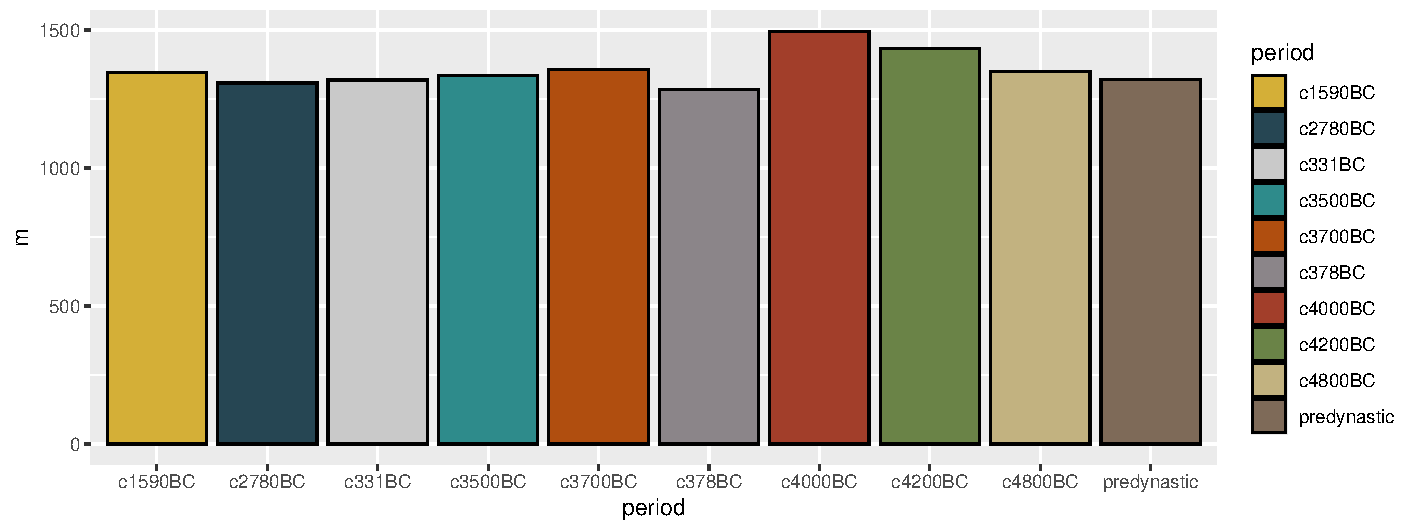
\includegraphics[width = 0.95\textwidth]{graphics/ch3Figs/bar_2.pdf}
\end{figure}

\subsection{Naming Levels}

On occasion, it will be useful to rename the levels of a factor. For instance, previously we had used the \R{labels} argument inside \textit{ggplot2}'s \R{scale\_x\_discrete()} function to adjust the \textit{x}-axis labelling. However, an alternative strategy would have been to relabel the factor levels. We can do this using the \R{levels()} function from earlier. And we have the option of renaming the levels of the \R{skulls} or \R{skull\_summary} data frames. We will do the latter so that we do not need to re-run the code that produced \R{skull\_summary}.

\begin{inR}
levels(skull_summary$period) <- c(
  "Predynastic", "c.4800 BC", "c.4200 BC", "c.4000 BC", "c.3700 BC",
  "c.3500 BC", "c.2780 BC", "c.1590 BC", "c.378 BC", "c.331 BC"
)
skull_summary
\end{inR}
\begin{outR}
# A tibble: 10 × 8
   period          m     n     N m_heq med_heq   min   max
   <fct>       <dbl> <int> <int> <dbl>   <dbl> <dbl> <dbl>
 1 Predynastic 1320.   318  1449 0.275   0.273  1050  1710
 2 c.4800 BC   1349.   124  1449 0.281   0.283  1110  1640
 3 c.4200 BC   1434.    16  1449 0.299   0.306  1110  1740
 4 c.4000 BC   1495.    50  1449 0.311   0.311  1235  1775
 5 c.3700 BC   1356.     7  1449 0.283   0.284  1245  1450
 6 c.3500 BC   1337.   315  1449 0.278   0.277   965  1760
 7 c.2780 BC   1308.   152  1449 0.273   0.270  1030  1660
 8 c.1590 BC   1347.   203  1449 0.281   0.280  1080  1665
 9 c.378 BC    1286.    32  1449 0.268   0.266  1095  1550
10 c.331 BC    1319.   232  1449 0.275   0.275  1000  1570
\end{outR}

\noindent
A corresponding change will be seen on the plot's \textit{x}-axis labels as well when that is generated.

\begin{inR}
ggplot(skull_summary, aes(x = period, y = m)) +
  geom_bar(stat = "identity") +
  labs(x = "Period", y = "Cranial Capacity (cm³)")
\end{inR}

\vspace{2em}

\begin{figure}[H]
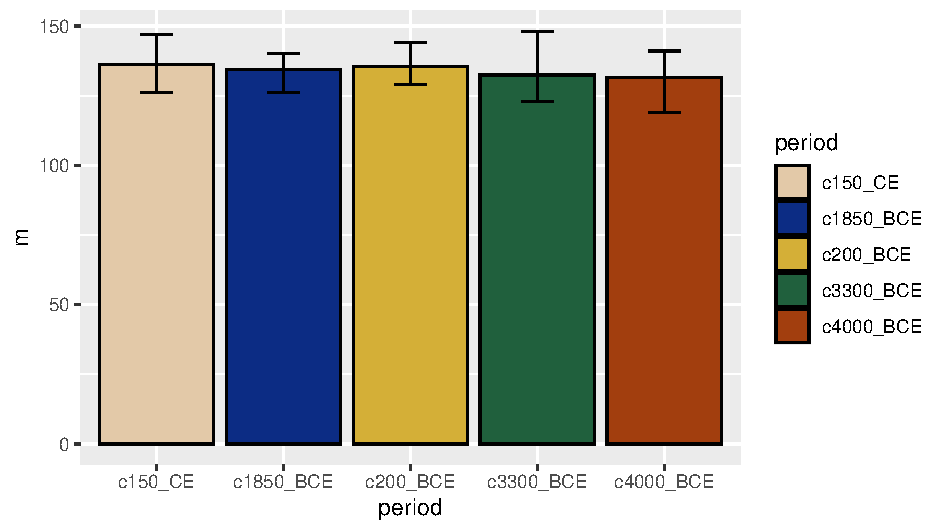
\includegraphics[width = 0.95\textwidth]{graphics/ch3Figs/bar_3.pdf}
\end{figure}

It would be remiss not to mention that \textit{ggplot2} provides a dedicated method for updating $x$-axis labels—one that doesn’t require modifying the factor levels directly. Specifically, you can use the \R{labels} argument within the \R{scale\_x\_discrete()} function. This approach simply involves supplying a character vector that specifies the new labels in their current plotting order, like so…

\begin{inRhigh}[highlightlines={4-8}]
ggplot(skull_summary, aes(x = period, y = m)) +
  geom_bar(stat = "identity") +
  labs(x = "Period", y = "Cranial Capacity (cm³)") +
  scale_x_discrete(
    labels = c(
      "Predynastic", "c.4800 BC", "c.4200 BC", "c.4000 BC", "c.3700 BC",
      "c.3500 BC", "c.2780 BC", "c.1590 BC", "c.378 BC", "c.331 BC"
      )
  )
\end{inRhigh}

Concerning the manipulation of factors, a brief word of warning is in order: \textbf{do not} confuse the \R{levels} \textit{argument} used inside the \R{factor()} function with the \R{levels()} \textit{function} itself. While they sound similar, they serve very different purposes.\footnote{To further complicate things (because of course it does), the \R{factor()} function also includes a \R{labels} argument that allows you to rename levels at the time of creation. See the R documentation for details: \R{?factor}}

\begin{itemize}
    \item \R{levels = ...} (argument inside \R{factor()}) is used to \textit{specify the order} of factor levels.
    \item \R{levels()} (function) is used to \textit{rename} existing factor levels.
\end{itemize}

For beginners, factors can feel particularly troublesome. But they are foundational to R's thaumaturgy and cannot be avoided. So rather than resisting, it is best to embrace their evil, arcane nature—otherwise you will never be at peace with yourself.

\section{Adding Error Bars}

Recall that in addition to the mean estimated cranial capacity for each period, \R{skull\_summary} also includes the smallest and largest measured capacities, stored in the \R{\$min} and \R{\$max} columns, respectively.

\begin{inR}
skull_summary
\end{inR}

\begin{outR}
# A tibble: 10 × 8
   period          m     n     N m_heq med_heq   min   max
   <fct>       <dbl> <int> <int> <dbl>   <dbl> <dbl> <dbl>
 1 Predynastic 1320.   318  1449 0.275   0.273  1050  1710
 2 c.4800 BC   1349.   124  1449 0.281   0.283  1110  1640
 3 c.4200 BC   1434.    16  1449 0.299   0.306  1110  1740
 4 c.4000 BC   1495.    50  1449 0.311   0.311  1235  1775
 5 c.3700 BC   1356.     7  1449 0.283   0.284  1245  1450
 6 c.3500 BC   1337.   315  1449 0.278   0.277   965  1760
 7 c.2780 BC   1308.   152  1449 0.273   0.270  1030  1660
 8 c.1590 BC   1347.   203  1449 0.281   0.280  1080  1665
 9 c.378 BC    1286.    32  1449 0.268   0.266  1095  1550
10 c.331 BC    1319.   232  1449 0.275   0.275  1000  1570
\end{outR}

\noindent
We can incorporate this information into our graph using \glspl{error bar}. Error bars provide a visual representation of the data's \textit{spread}, and the difference between the maximum and minimum values corresponds to a classic measure of spread known as the \textit{range}.\footnote{If this concept isn’t entirely clear yet, don’t worry—spread, as a formal statistical idea, will be explored in more detail in later chapters.} While the range is generally not recommended as a primary measure of spread, it has the advantage of being intuitive and serves our current illustrative purposes well enough.

To create error bars, we can simply use \textit{ggplot2's} \R{geom\_errorbar()} function. We just need to tell it which column corresponds to the bottom of the error bars, using the argument \R{ymin}, and which column corresponds to the top of the error bars, using the argument \R{ymax}.

\begin{inRhigh}[highlightlines={3}]
ggplot(skull_summary, aes(x = period, y = m)) +
  geom_bar(stat = "identity") +
  geom_errorbar(aes(ymin = min, ymax = max), width = 0.25) +
  labs(x = "Period", y = "Cranial Capacity (cm³)")
\end{inRhigh}

\vspace{2em}

\begin{figure}[H]
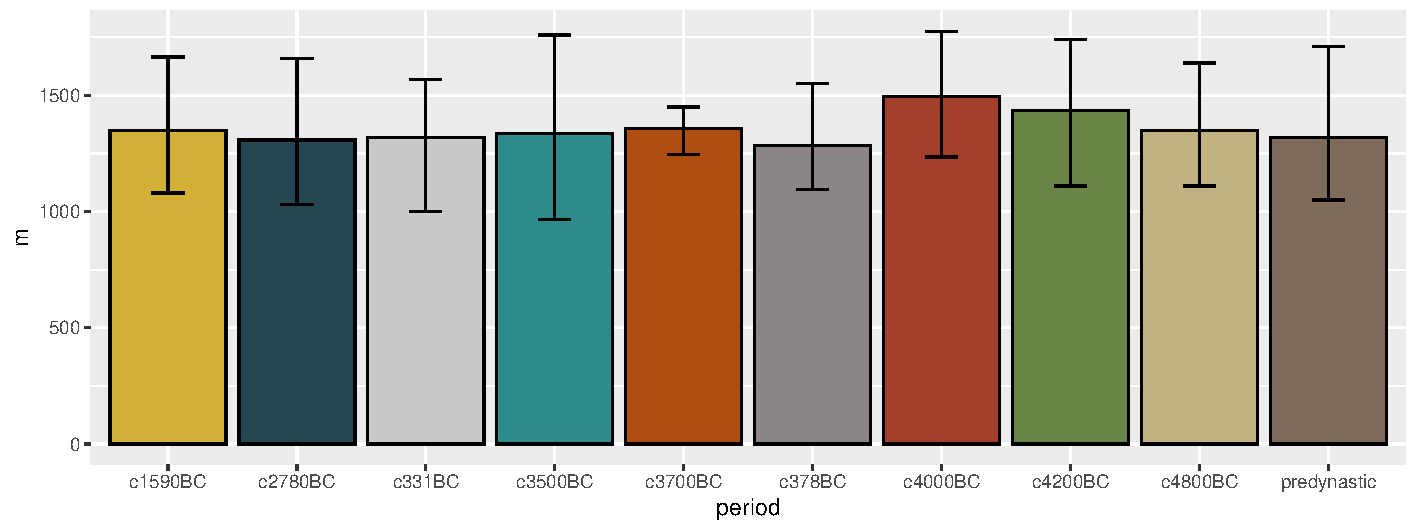
\includegraphics[width = 0.95\textwidth]{graphics/ch3Figs/bar_4.pdf}
\end{figure}

\section{Bar Fill Colour}

To further enhance the bar plot's visual appeal, we could adjust the fill colour of the bars to reflect the corresponding time periods.

But we should pause for a moment because, strictly speaking, this is something we should NOT do—unless we have a compelling reason. And in this case, we do not have a compelling reason. The purpose of a plot like this is to compare the heights of the bars—that is, the $y$-axis values. From a scientific standpoint, it’s best to ensure that each bar has equal visual weight, and using a single consistent colour accomplishes exactly that. Since the categories are already labelled on the $x$-axis, additional colours only serve as unnecessary distractions that might bias or obscure the comparisons you are trying to see. For instance, something like this would be scientifically acceptable:

\begin{inRhigh}[highlightlines={2}]
ggplot(skull_summary, aes(x = period, y = m)) +
  geom_bar(stat = "identity", colour = "black", fill = "#CBA135") +
  geom_errorbar(aes(ymin = min, ymax = max), width = 0.25) +
  labs(x = "Period", y = "Cranial Capacity (cm³)")
\end{inRhigh}

\vspace{2em}

\begin{figure}[H]
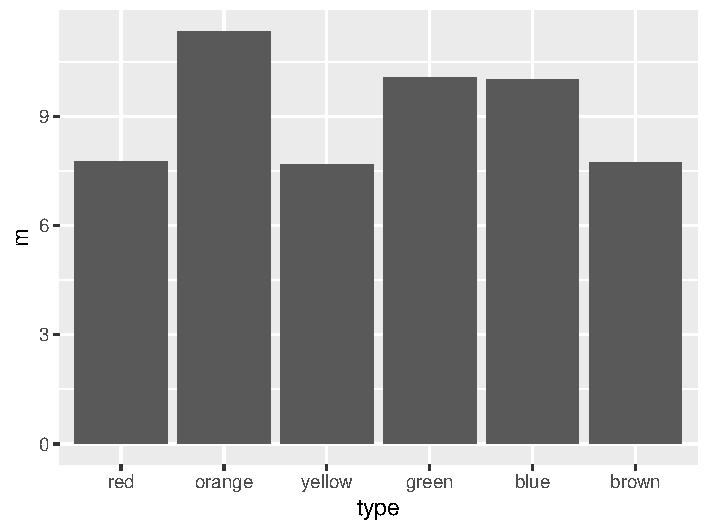
\includegraphics[width = 0.95\textwidth]{graphics/ch3Figs/bar_5.pdf}
\end{figure}

That said, if you’re collaborating on a project, your teammates may insist on rainbow-coloured bars or other such nonsense regardless of this sound logic. And if they outnumber you, they’ll win the vote—and possibly the fistfight. Science offers no defence against the tyranny of \mbox{``aesthetics.''}

Setting aside everything we just said, if we do decide to adjust the colour of the bars, we need to be mindful of how the $x$-axis is structured. Technically, the $x$-axis represents a \textit{discrete} scale—not a \textit{continuous} one (see Section \ref{sec:pos_scale} for more on this distinction). However, while \textit{ggplot2} treats it as discrete (because it's a bar plot), the underlying variable—ordered time periods—does follow a natural continuum theoretically. So, in this case, using a continuous colour palette is not entirely unjustified. To that end, we can make use of one of R’s many HCL palettes discussed in Section \ref{sec:hcl_palettes}. The ``Green-Brown'' palette, in particular, is a solid choice—it provides a smooth gradation that maps well onto temporal data without being garish or overly distracting.\footnote{A visual guide to all HCL palettes is available in Appendix \ref{sec:AppendixPalettes}.}

Given that we have 10 separate categories of dates, we can define our palette in the following way.\footnote{If you want to be a bit fancy—and make your code more robust—you can write something like \R{egypt\_pal <- hcl.colors(\textbf{length(levels(skulls\$period))}, palette = "Green-Brown")}. This way, if you ever remove levels, the number of colours will automatically adjust, and you won’t need to revise your code manually.}

\begin{inR}
egypt_pal <- hcl.colors(n = 10, palette = "Green-Brown")
\end{inR}

\clearpage

\noindent
We can then use \R{egypt\_pal} to adjust the fill colour of the bars in the plot.

\begin{inRhigh}[highlightlines={2,5}]
ggplot(skull_summary, aes(x = period, y = m)) +
  geom_bar(stat = "identity", colour = "black", aes(fill = period)) +
  geom_errorbar(aes(ymin = min, ymax = max), width = 0.25) +
  labs(x = "Period", y = "Cranial Capacity (cm³)") +
  scale_fill_manual(values = egypt_pal)
\end{inRhigh}

\vspace{2em}

\begin{figure}[H]
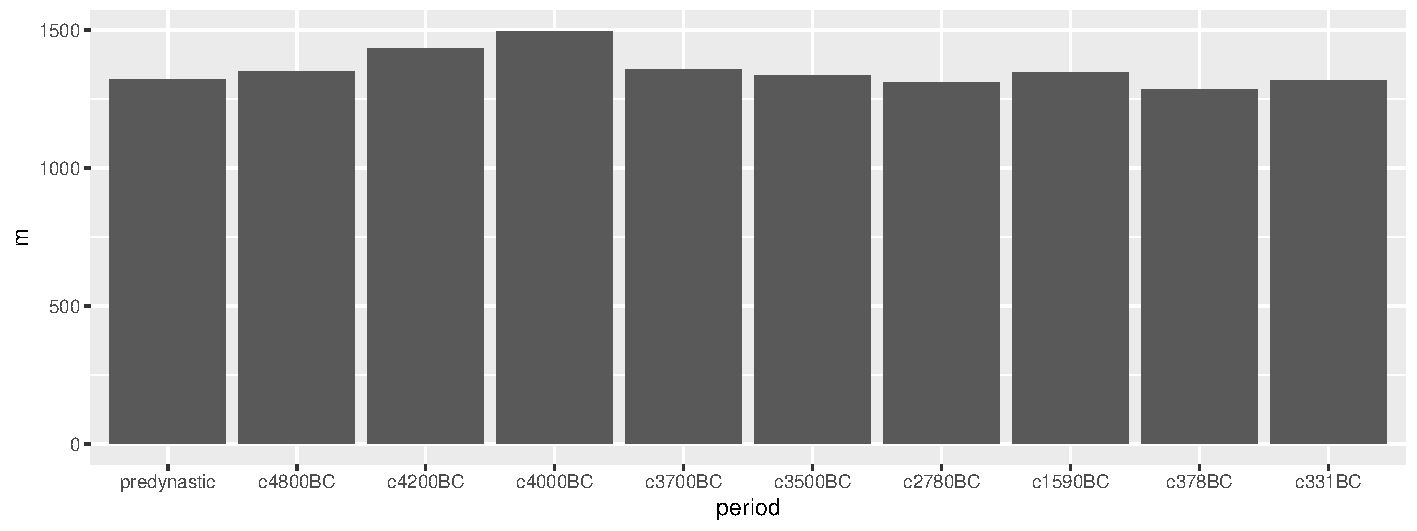
\includegraphics[width = 0.95\textwidth]{graphics/ch3Figs/bar_6.pdf}
\end{figure}

\noindent
\textit{ggplot2} quite sagely adds a legend when you map fill colours to a variable; however, in this particular case the legend is redundant with the information our \textit{x}-axis provides and is thus taking up space unnecessarily. To remove the legend, there are different methods that could be employed. Since we only have the fill aesthetic mapped, it is easy enough to just add \R{guide = "none"} to the \R{scale\_fill\_manual()} function.

\begin{inRhigh}[highlightlines={5}]
ggplot(skull_summary, aes(x = period, y = m)) +
  geom_bar(stat = "identity", colour = "black", aes(fill = period)) +
  geom_errorbar(aes(ymin = min, ymax = max), width = 0.25) +
  labs(x = "Period", y = "Cranial Capacity (cm³)") +
  scale_fill_manual(values = egypt_pal, guide = "none")
\end{inRhigh}

\vspace{2em}

\begin{figure}[H]
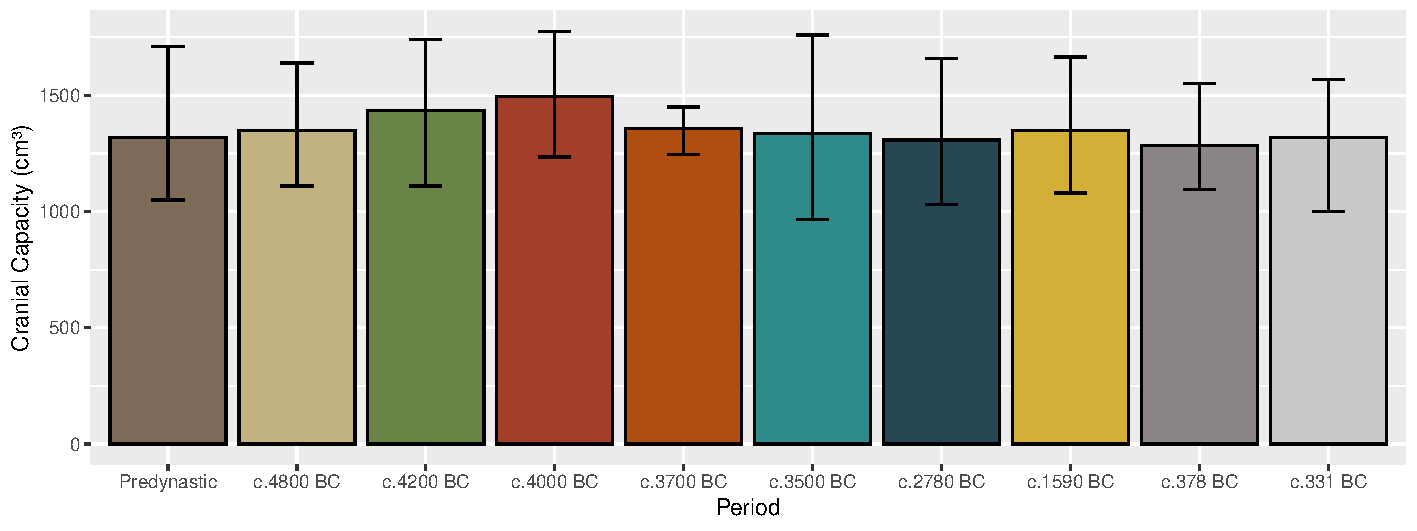
\includegraphics[width = 0.95\textwidth]{graphics/ch3Figs/bar_7.pdf}
\end{figure}

\section{Putting It All Together}

To consolidate everything covered in this chapter, it's helpful to revisit the analysis one final time—but in a more realistic, streamlined, end-to-end format. Doing so not only reinforces how the various components work together in a complete R script, but also provides an opportunity to enhance the graph by incorporating some faceting\footnote{Facets were covered in Chapter 2, section \ref{sec:facets}.} based on the previously ignored variable \R{\$sex}.

\begin{inR}
# Load the tidyverse (and praise the our dear leader Hadley)
library(tidyverse)
\end{inR}

\begin{inR}
# Load the data
skulls <- read_csv("skull_cap_partial_wide.csv") |>
  # Pivot to the tidy format
  pivot_longer(
    cols = predynastic:c331BC,
    names_to = "period",
    values_to = "capacity"
  ) |>
  # Remove NAs
  drop_na(capacity)
\end{inR}

\begin{inR}
# Factor and order "period"
skulls$period <- factor(skulls$period,
  levels = c(
    "predynastic", "c4800BC", "c4200BC", "c4000BC", "c3700BC",
    "c3500BC",     "c2780BC", "c1590BC", "c378BC",  "c331BC"
  )
)
\end{inR}

\begin{inR}
# Rename the factor levels
levels(skulls$period) <- c(
  "Predynastic", "c.4800 BC", "c.4200 BC", "c.4000 BC", "c.3700 BC",
  "c.3500 BC",   "c.2780 BC", "c.1590 BC", "c.378 BC",  "c.331 BC"
)
\end{inR}

\begin{inRhigh}[highlightlines={3}]
# Calculate stats for plot, grouping by 'period' and 'sex'
skull_summary <- skulls |>
  group_by(period, sex) |> # Note the addition of a second factor to group_by()
  summarise(
    m = mean(capacity),
    min = min(capacity),
    max = max(capacity)
  )

skull_summary # Output shows group-wise means and ranges, separated by sex
\end{inRhigh}

\begin{outR}
# A tibble: 18 × 5
# Groups:   period [10]
   period      sex        m   min   max
   <fct>       <chr>  <dbl> <dbl> <dbl>
 1 Predynastic Female 1262.  1050  1570
 2 Predynastic Male   1391.  1130  1710
 3 c.4800 BC   Female 1280.  1110  1515
 4 c.4800 BC   Male   1430.  1195  1640
 5 c.4200 BC   Female 1271   1110  1530
 6 c.4200 BC   Male   1509.  1320  1740
 7 c.4000 BC   Male   1495.  1235  1775
 8 c.3700 BC   Female 1356.  1245  1450
 9 c.3500 BC   Female 1255.   965  1490
10 c.3500 BC   Male   1408.  1160  1760
11 c.2780 BC   Female 1252.  1030  1520
12 c.2780 BC   Male   1384.  1160  1660
13 c.1590 BC   Female 1288.  1080  1515
14 c.1590 BC   Male   1421.  1210  1665
15 c.378 BC    Female 1227.  1095  1400
16 c.378 BC    Male   1345.  1190  1550
17 c.331 BC    Female 1245   1000  1455
18 c.331 BC    Male   1383.  1150  1570
\end{outR}

\begin{inR}
# Store desired colours
egypt_pal <- hcl.colors(n = 10, palette = "Green-Brown")
\end{inR}

\clearpage

\begin{inRhigh}[highlightlines={14}]
# Plot data
ggplot(skull_summary, aes(x = period, y = m)) +
  geom_bar(
    stat = "identity",
    colour = "black",
    aes(fill = period)
  ) +
  geom_errorbar(aes(ymin = min, ymax = max), width = 0.25) +
  scale_fill_manual(values = egypt_pal, guide = "none") +
  labs(
    x = "Period",
    y = "Cranial Capacity (cm³)"
  ) +
  facet_wrap(~ sex, ncol = 1) # Note the use of facet_wrap
\end{inRhigh}

\vspace{2em}

\begin{figure}[H]
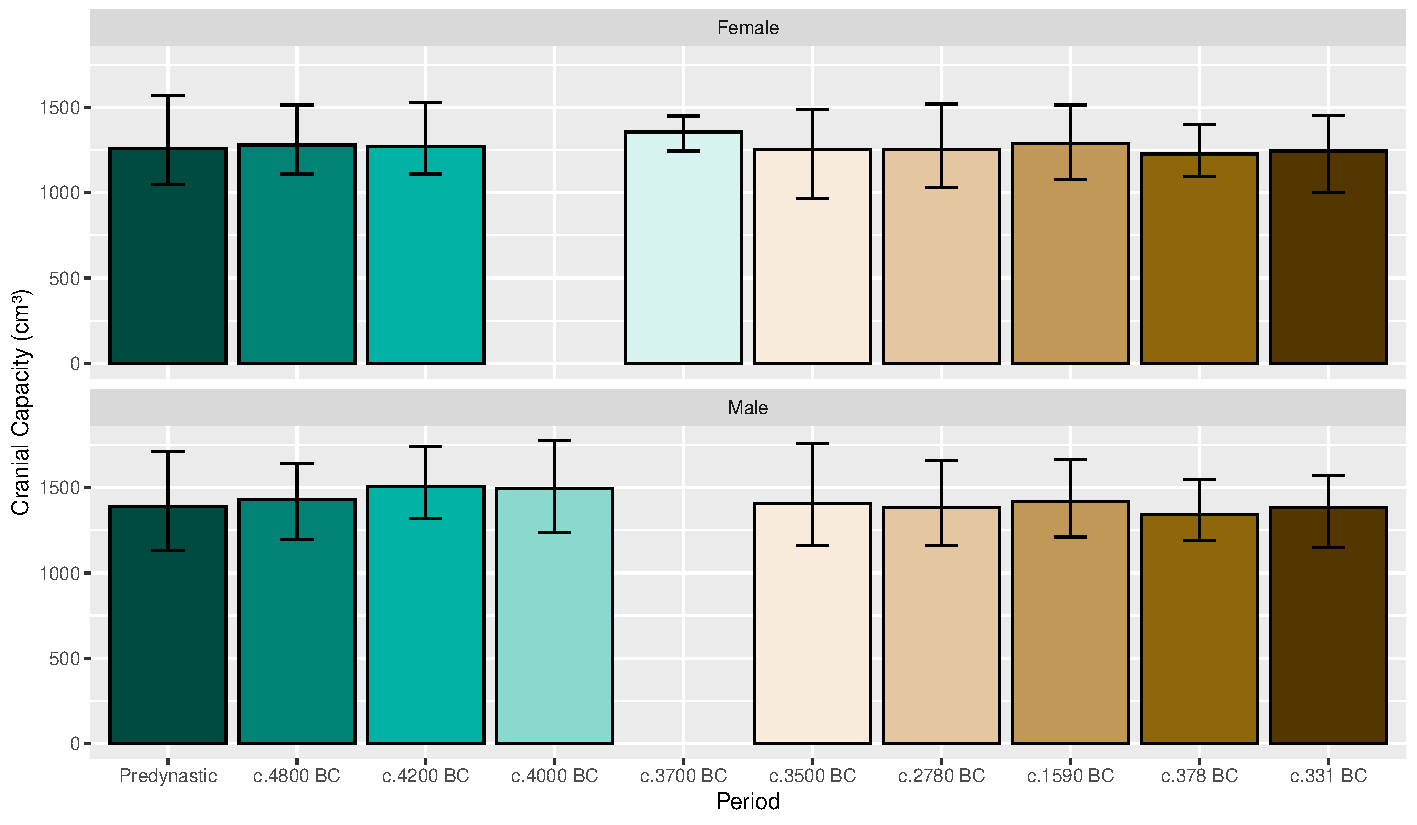
\includegraphics[width = 0.95\textwidth]{graphics/ch3Figs/bar_8.pdf}
\end{figure}

\clearpage

Finally, it is worth demonstrating just how easily—and dramatically—we can adjust \textit{ggplot2} to suit different analytical goals. As it currently stands, the plot is structured to compare cranial capacity across time periods within each sex. However, with just two minor changes (see line 2 and 14), we can reorient the layout to instead compare the sexes within each time period. Specifically, we place \R{\$sex} on the $x$-axis and facet according to \R{\$period}.

%\footnote{While the data shows that males tend to have slightly larger crania on average, it's worth noting that the sperm whale (\textit{Physeter macrocephalus}) possesses a brain over five times the size of a human’s—and yet it spends much of its time ramming giant squid in total darkness and clicking at 230 decibels. Don't over-interpret this finding. Male skulls may be bigger on average—but before anyone gets too proud, remember: it's what you do with your brain that counts.}

\begin{inRhigh}[highlightlines={14}]
# Plot data
ggplot(skull_summary, aes(x = sex, y = m)) +
  geom_bar(
    stat = "identity",
    colour = "black",
    aes(fill = period)
  ) +
  geom_errorbar(aes(ymin = min, ymax = max), width = 0.25) +
  scale_fill_manual(values = egypt_pal, guide = "none") +
  labs(
    x = "Sex",
    y = "Cranial Capacity (cm³)"
  ) +
  facet_wrap(~ period, ncol = 5)
\end{inRhigh}

\vspace{2em}

\begin{figure}[H]
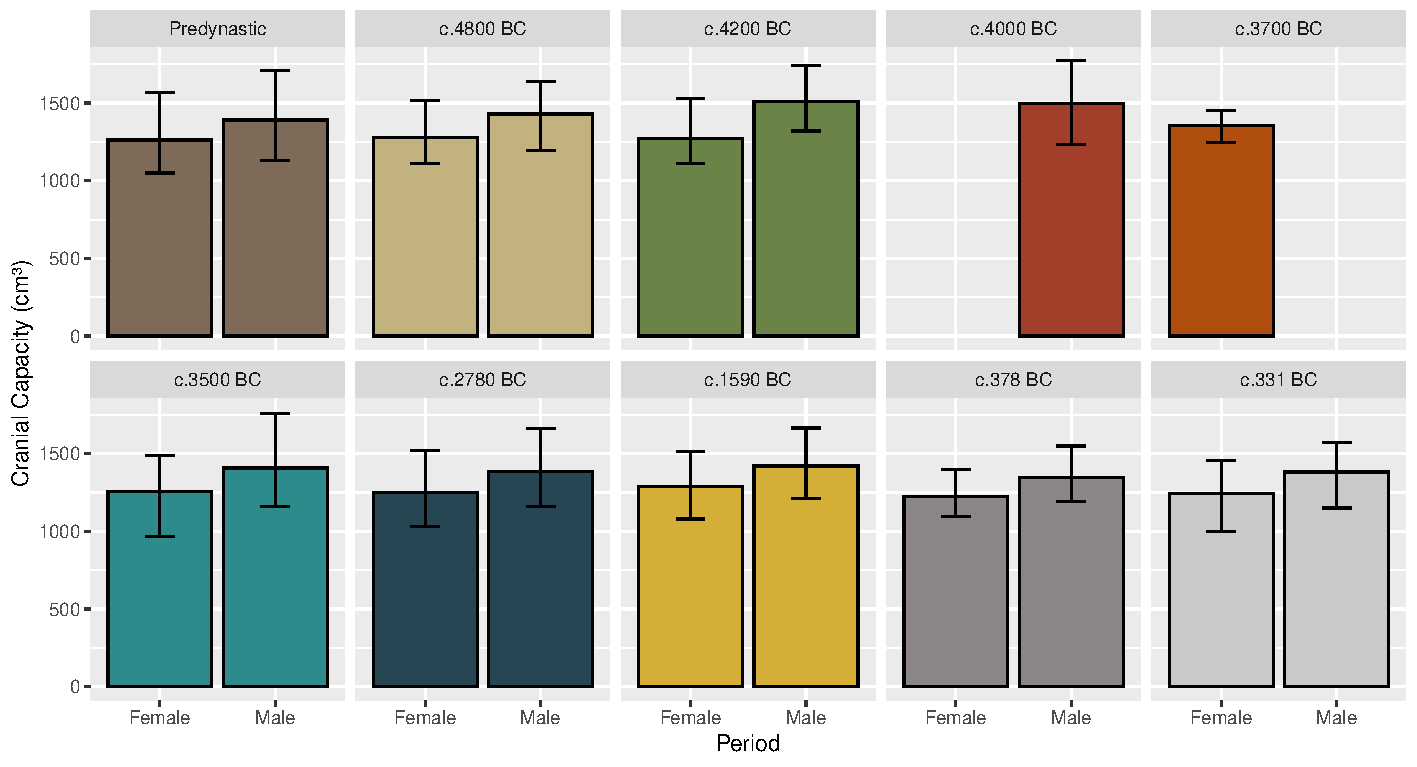
\includegraphics[width = 0.95\textwidth]{graphics/ch3Figs/bar_9.pdf}
\end{figure}
